\documentclass[12pt]{article}
\usepackage{a4}
\usepackage[english]{babel}
\setlength{\parindent}{0.35cm}
\pagestyle{headings}
\usepackage{graphicx}
%Multiple picture in one figure
%\usepackage{subfigure}
\usepackage{listings}
\usepackage{color}
%Zum Zeilen umbrechen in Tabellen
\usepackage{pbox}
\usepackage{wrapfig}
%Floating-Umgebungen
\usepackage{float}
%Math-Environment
\usepackage{amsmath}
%Better SI-Units
\usepackage{siunitx}
\DeclareSIUnit\century{century}
\DeclareSIUnit\year{yr}
%Using Appendix
\usepackage[title]{appendix}
%Using URL
\usepackage[hidelinks]{hyperref}
%Using Colored Tables
\usepackage{colortbl}
%Use subfigs
\usepackage{subfig}
%Configure geometry
\usepackage{geometry}
%\geometry{
%	a4paper,
%	left=3cm,
%	right=3cm,
%	top=3cm,
%	bottom = 3cm,
%	}

\lstset{
	language=C++,
	basicstyle=\small\ttfamily,
	keywordstyle=\color{blue}\ttfamily,
	stringstyle=\color{red}\ttfamily,
	commentstyle=\color{green}\ttfamily,
	morecomment=[l][\color{magenta}]{\#},
}

\usepackage{booktabs}
\sisetup{
	per-mode=fraction,
	%	fraction-function=\tfrac
}

% New/Renewing Commands
\newcommand{\eV}{\electronvolt}
\newcommand{\keV}{\kilo\electronvolt}
\newcommand{\meV}{\mega\electronvolt}
\newcommand{\gray}{\rowcolor[gray]{.90}}
\newcommand{\degr}{^{\circ}}
\newcommand{\tit}[1]{\textit{#1}}
\newcommand{\baf}{BaF$_2$}
\newcommand{\pwo}{PbWO$_4$}
\newcommand{\ten}[1]{$10^{#1}$}
\newcommand{\orb}[2]{$#1^{#2}$}
\newcommand{\stat}[2]{$#1_{#2}$}
\newcommand{\ft}[2]{$#1\rightarrow#2$}
\newcommand{\sr}{$^{90}$Sr}
\newcommand{\co}{$^{60}$Co}
\newcommand{\eu}{$^{152}$Eu}
\newcommand{\cs}{$^{137}$Cs}
\newcommand{\ba}{$^{133}$Ba}
\newcommand{\na}{$^{22}$Na}
\newcommand{\ka}{$^{40}$Ka}


\begin{document}
	
	\title{
		\textbf{Development of a SiPM-based readout-module for the characterization of various scintillator materials \textcolor{red}{READABLE one-column version} }
	}
	\author{Lukas Nies}
	\date{\today	
	}
	\clearpage\maketitle\thispagestyle{empty}

	\setcounter{page}{0}

In this paper we discuss a general approach to use SiPMs in different electrical configurations in combination with numerous scintillator materials for applications in nuclear instrumentation, like calorimetry and timing. The "hybrid" configuration used in the PANDA detector was found to show fastest timing properties with several hundred $\si{\pico\second}$ response by combining the advantages of a large active area while avoiding high operation voltages and dark noise. A "parallel" configuration shows the largest light collection efficiency and is therefore suitable for energy measurements. Several calibration spectra were taken to measure the energy deposit of minimal ionizing cosmic muons in a $2\si{\centi\meter}$ thick \pwo{} crystal. \textcolor{red}{WORK IN PROGRESS} \par 
Modern photodetector applications encounter a large spectrum of different experimental environments. Prerequisites, e.g. working within strong magnetic fields, providing large intrinsic amplification, independence on high operation voltage, and space restrictions lead to the development of a new type of detectors, the semiconductor diodes. The \tit{Silicon Photomultiplier} (SiPM) integrates a large number of \tit{avalanche photodiodes} as microcells within a small space. With a large intrinsic amplification of up to $10^6$, the SiPM comes in many different packaging sizes and works mainly with low voltage between $\SI{25}{\volt}$ and $\SI{85}{\volt}$. Its insensitivity to magnetic fields and single photon counting capability in combination with suited scintillators make SiPMs a valuable choice for modern challenging applications, i.e. \tit{nuclear magnetic resonance imaging}, \tit{positron emission tomography}, and high energy calorimetry and tracking. \\ \indent
The development of the scintillation tile hodoscope \cite{SciTil}, short SciTil, for the \tit{PANDA} detector at the future Facility for Antiproton and Ion Research (\tit{FAIR}) at the GSI Helmholtz Centre for Heavy Ion Research in Germany \cite{FAIR} necessitated the development of a small-scale photo readout system insensitive to the magnetic field of the detector. The Wien group chose SiPMs due to previously mentioned properties. Coupling multiple SiPMs in an array increases the effective active area and, thus, enhances the photon detection efficiency. \\ \indent
\begin{figure}[b!]
	\centering
	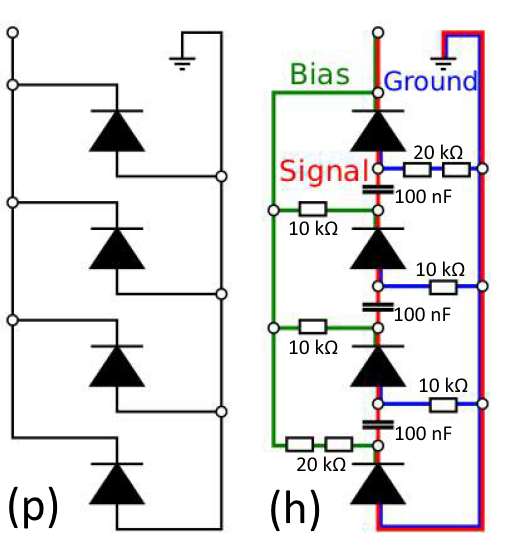
\includegraphics[width=0.5\linewidth]{./graphics/ch4/circuits.PNG}
	\caption{ Schematic of the two different SiPM configurations \cite{sebastian}. On the left is the ``parallel" configuration, on the right is the ``hybrid" configuration. The signal path is depicted in red, the bias current in green, and the ground in blue.  }
	\label{fig:PCB}
\end{figure}
In order to develop a general purpose SiPM array we designed in first iteration a printed circuit board (\tit{PCB}) which is able to host either a "parallel" or "hybrid" configuration by just adding or removing some resistors and capacities on the back of the board (see figure \ref{fig:PCB}). The signal is read out via a "bias-T" consisting of a resistor and a capacity which decouple the signal from the DC biasing.  \\ \indent
Attached to a plastic scintillator, comparing the raw and normalized signal shapes of a single SiPM with an array of four diodes in either parallel or hybrid configuration shows the fundamental differences of the methods. The signal amplitude for the hybrid configuration is roughly $\frac{1}{\sqrt{N}}$ compared to the amplitude of a single SiPM, where $N$ stands for the number of SiPMs per array. Driving the SiPM in parallel mode does not affect the signal amplitude. With a few nanoseconds the hybrid configuration has a considerably faster rising edge in respect to the parallel configuration where the latter tends to get slower as the number of SiPMs per array increases. Hence, SiPM-arrays in hybrid configuration are more suitable for time measurements whereas the parallel configuration is useful for energy measurements. \\ \indent
In order to yield breakdown and operation voltages, the temperature dependent current-voltage characteristics were studied. For this, the different configurations were wrapped with opaque tape to prevent occurrence of photon induced currents and put in a programmable refrigerator. For different temperatures between $-25^{\circ}C $ and $25^{\circ}C$ the SiPM-boards were biased and the IV-curves were measured with a custom made high voltage distribution board designed for operating the avalanche photo diodes of the electromagnetic calorimeter barrel of the PANDA detector \cite{chris}. \\ \indent
If a photo diode is driven in reversed bias mode the depletion layer between the p- and n-junction broadens and the built-in potential intensifies. At the breakdown voltage $U_{BD}$ electrons gain sufficient energy to create a self-sustained avalanche which leads to an exponential increase in current flowing. The breakdown voltages was determined by the intersection of a first order polynomial fit for the voltage area before breakdown and a second order polynomial for the region right after breakdown. \\ \indent
In order to find the optimal operation voltage $U_{OP}$, which is usually a few volts beyond breakdown, the minimum of the relative slope $\frac{dI}{dV}\frac{1}{I(V)}$ of the IV-curve was fitted. \\ \indent 
After scanning the IV-characteristics at different temperatures, the resulting breakdown temperature coefficient $k_{BD}$ for a single SiPM was in good agreement with the specifications of the manufacturer \cite{SiPM_Manual} (see \ref{tab:IV_cata}). The value for multiple SiPM does not seem to change (within the error). The coefficient for the operation voltage seems to add as the number of SiPMs increases: the four-SiPM array has a roughly four times higher values as the single SiPM. \\ \indent
\begin{table}[t!]
	\centering
	\begin{tabular}{ c|cc|cc } \toprule[2pt]
		& \multicolumn{2}{c|}{(s)-configuration} & \multicolumn{2}{c}{(h)- and (p)-configuration} \\
		T [$\si{\degreeCelsius}]$ & $V_{OP}$ [$\si{\volt}$] & $V_{BD}$ [$\si{\volt}$] & $V_{OP}$ [$\si{\volt}$] & $V_{BD}$ [$\si{\volt}$]  \\ \midrule
		-25 & $30.78\pm 3.99$ & $24.62\pm 2.89$ & $30.72\pm 0.47$ & $24.40\pm 3.67$ \\
		0 & $30.67\pm 0.42$ & $25.50\pm 0.60$ & $30.89\pm 0.15$ & $24.78\pm 0.03$ \\
		5 & $30.72\pm 0.32$ & $24.93\pm 0.15$ & $31.01\pm 0.59$ & $24.87\pm 0.04$ \\
		10 & $30.70\pm 0.35$ & $25.11\pm 0.44$ & $31.20\pm 0.32$ & $25.04\pm 0.04$ \\
		15 & $30.74\pm 0.28$ & $25.30\pm 0.14$ & $31.32\pm 0.68$ & $25.08\pm 0.01$ \\
		20 & $30.80\pm 0.23$ & $25.35\pm 0.05$ & $31.57\pm 0.75$ & $25.18\pm 0.03$ \\
		25 & $30.87\pm 0.45$ & $25.51\pm 0.23$ & $31.04\pm 2.11$ & $25.20\pm 0.06$ \\
		\midrule
		& $k_{OP}$ [$\si{\milli\volt\per\kelvin}$] & $k_{BD}$ [$\si{\milli\volt\per\kelvin}$] & $k_{OP}$ [$\si{\milli\volt\per\kelvin}$] & $k_{BD}$ [$\si{\milli\volt\per\kelvin}$]  \\
		& $6.79\pm 1.34$ & $23.66\pm 5.10$ & $23.67\pm 2.90$ & $19.30\pm 1.51$ \\
		\bottomrule[2pt]
	\end{tabular}
	\caption[Fit results for operation and breakdown voltages]{Fit results for operation and breakdown voltages. Since the same SiPMs were used for (h)- and (p)-configuration the results are similar.}
	\label{tab:IV_cata}
\end{table}  
Since the diode is driven some volts beyond breakdown a probability is given that an avalanche is triggered by high energetic seed electrons. Because a SiPM is made up of thousands of microcells it is very likely to have plenty breakdowns in parallel every second. This effect can be suppressed by cooling where the high energetic part of the Boltzmann distributed electrons in the depletion layer gets shifted to lower thermal energies. \\ \indent
\begin{figure}[b!]
	\centering
	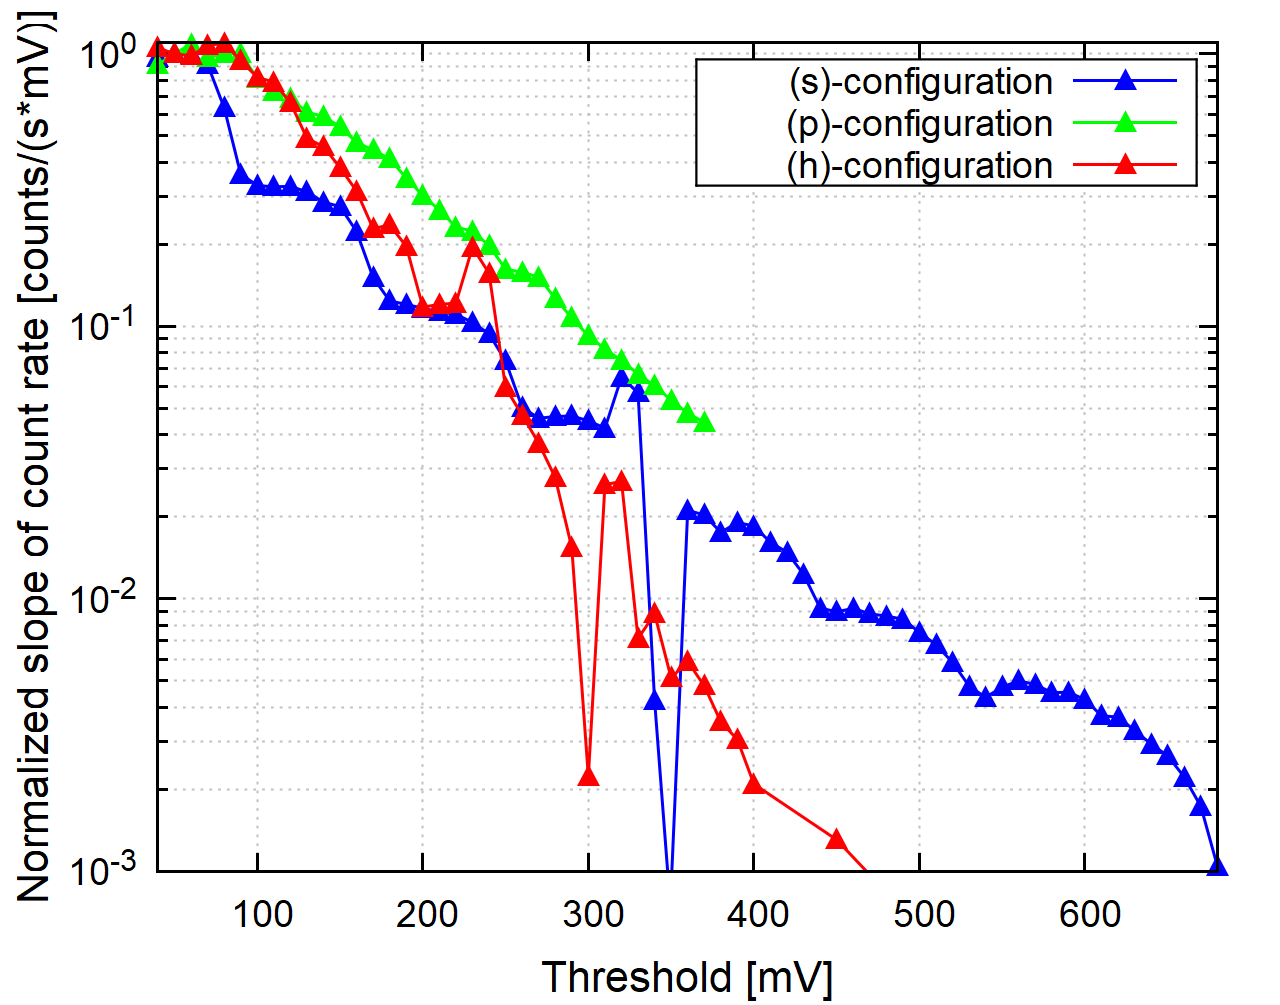
\includegraphics[width=0.9\linewidth]{./plots/dark_electron_spectrum/slope_countrate.png}
	\caption{Normalized slope of the dark count rate (note the logarithmic scale). The distinct step-like behavior for a single SiPM (blue) is clearly visible, while this subtle effect vanishes for multiple SiPMs (hybrid in red, parallel in green).}
	\label{fig:dark_count_rate}
\end{figure} 
Examining this so-called dark count rate (signal without seeing a photon) of SiPMs is crucial for light sensitive applications. It is not recommended using SiPMs at room temperature for single photon counting since the dark count rate is high. By deploying different diode configurations in an opaque box and measuring the pulse height spectrum behind a pre-amplifier with an oscillator in persistence mode we investigated the dependence of count rate and threshold. For better visibility of this effect, the normalized dark count rate for different configurations is depicted in figure \ref{fig:dark_count_rate}. Because every microcell, if firing, contributes the same signal to the overall signal a single SiPM shows a step-like behavior for increasing thresholds. The possibility of three cells firing at the same time is suppressed by a factor of ten, and for six cells the suppression is almost a factor of hundred. In our setup, this effect can not be seen for multiple SiPMs. Every diode is biased by the same voltage but each SiPM has slightly different gain, therefore the pulse heights smear and a threshold scan does not yield a step-like drop of count rate. \\ \indent
Hence, for precise measurements with SiPMs at scintillators with low expected light yield, it is necessary to match diodes per array withc comparable gain and to cool the detector for lower noise. \\ \indent
In order to examine the timing properties of the configurations a plastic scintillator \tit{EJ-248M} from \tit{ELJEN} with sizes $\SI{25.50}{\centi\meter}\times\SI{12.25}{\centi\meter}\times\SI{5}{\milli\meter}$ was cut (for geometry see figure \ref{fig:timing}), wrapped in layers of Teflon, aluminum, and finally in thick, opaque foil. Two opposite sides, which has been designed to have the same area as the SiPM-boards, were left uncovered. For spacing, the boards were equipped with a rubber mask with reflective foil leaving the SiPMs uncovered. For detailed descriptions see \cite{Lukas_Thesis}. This design was chosen for measuring cosmic muons for the project \tit{Cosmic Radiation: Measuring Cosmic Muons with the Raspberry Pi} \cite{schauer_projekt}, because this shape provides a large area with a ``pseudo" light-guide towards the narrow edges where the SiPM boards were attached. Optical grease was used to ensure good light transmission between scintillator material and SiPM entrance window. \\ \indent 
First, the raw signals of the boards were examined. A "bias-T" \cite{Lukas_Thesis} decouples the AC signal from the DC biasing. Afterwards, pre-amplifier from \tit{Phtotnique} \cite{photonique} were used for signal shaping. The results can be seen in figure \ref{fig:signals}. \\ \indent
\begin{figure}[t!]
	\subfloat[Raw signal of the different configurations: blue (4x1 hybrid), red (4x1 parallel), green (1x1 single)] {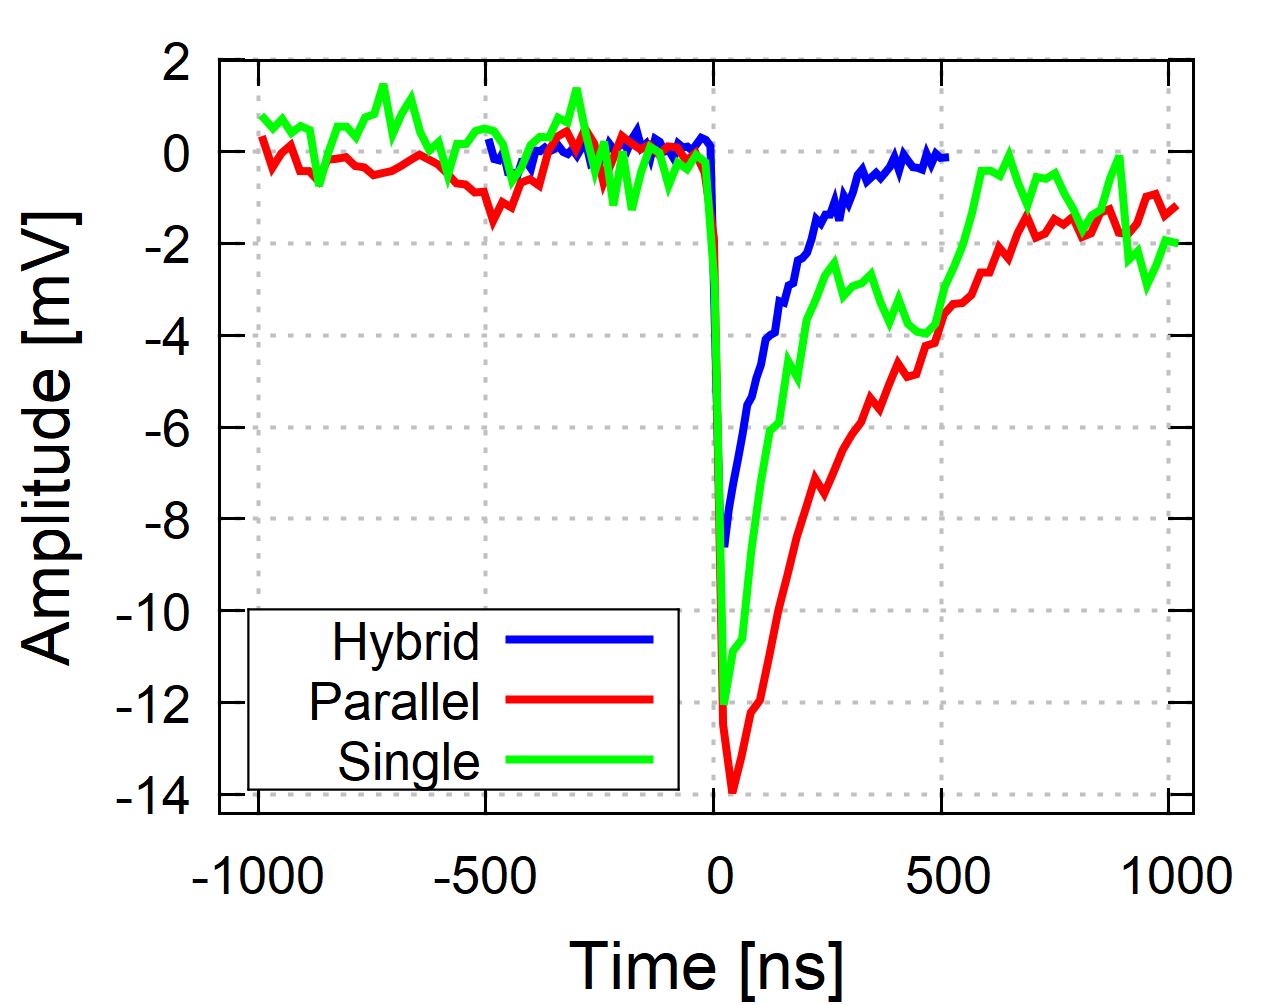
\includegraphics[width=0.49\textwidth]{./plots/signal/raw_large.png}}
	\hfill
	\subfloat[Amplified and normalized signal of blue (4x1 hybrid), red (4x1 parallel), green (1x1 single) with utilized photonique preamplifier] {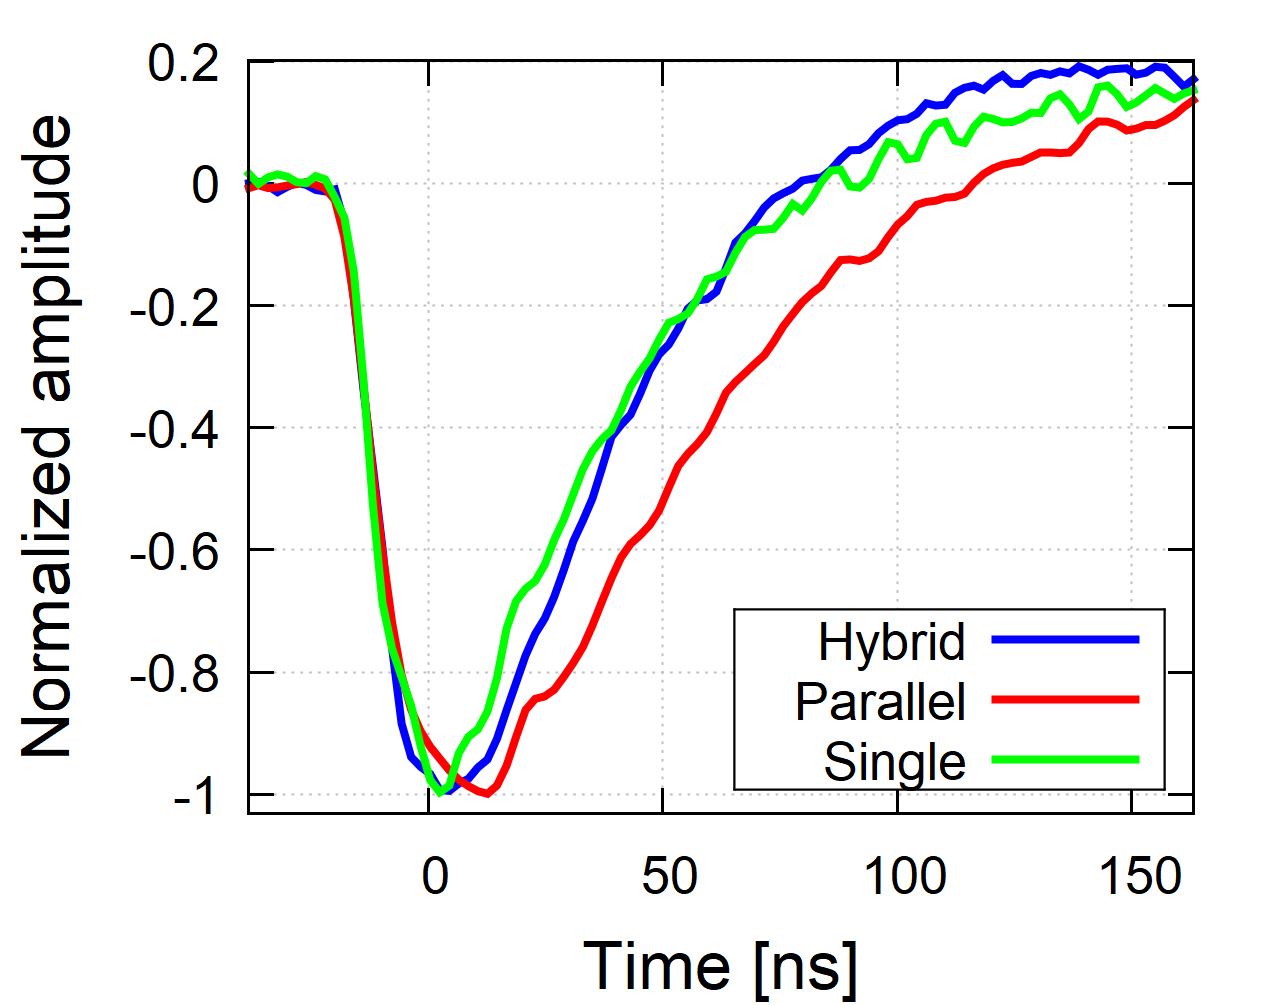
\includegraphics[width=0.49\textwidth]{./plots/signal/amp_large.png}}
	\hfill
	\caption{Raw and amplified signals of different SiPM configurations.}
	\label{fig:signals}
\end{figure}
As mentioned above, the signal strength depends on the number of SiPMs per board and on the configuration. The amplitude for the hybrid configuration gets divided by the square root of number of SiPMs utilized in the circuit where the parallel configuration has the same strength as a single SiPM. When using a preamplifier and normalizing the spectra one can see that the rise time of the hybrid board is fastest and the parallel board is slowest. Again, this suggests the use of hybrid boards for timing. \\ \indent
In preparation for the timing measurement the efficiency in counting and symmetry was tested. For this, two hybrid boards were mounted on each side of the scintillator and were connected via preamplifiers to a leading edge discriminator. The output of those two channels were fed into a counter which was controlled by an external clock. A third channel was used to count the coincident counts of channel one and two. The threshold of the leading edge discriminator was set for both channels to account for the expected rate of cosmic muons in the scintillator. A \sr source with a small collimator was placed on several areas on top of the scintillator to create photoelectrons. \\ \indent
\begin{figure}[b!]
	\subfloat[Measurement positions] {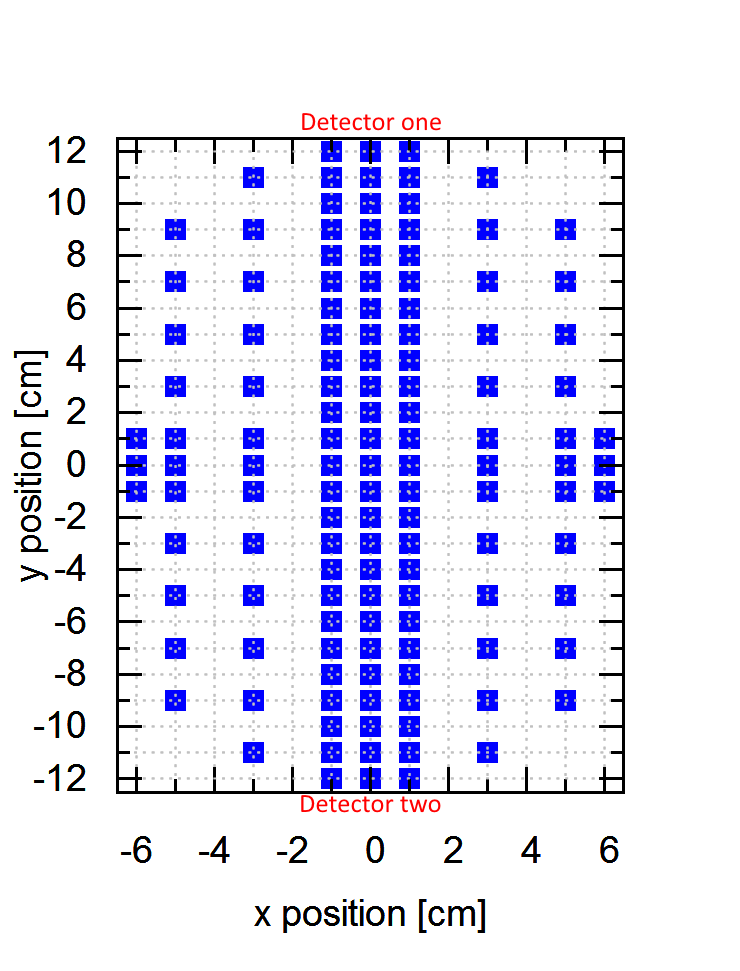
\includegraphics[width=0.24\textwidth]{./plots/spatial/aufnahme_punkte.png}}
	\hfill
	\subfloat[Detector one] {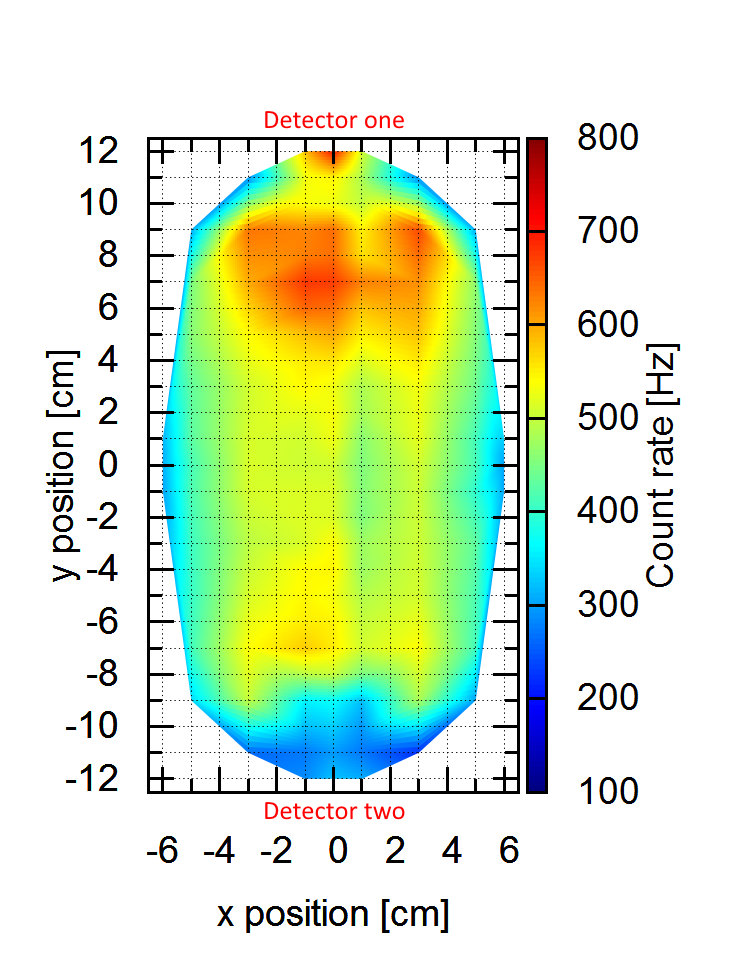
\includegraphics[width=0.24\textwidth]{./plots/spatial/Det1.png}}
	\hfill
	\subfloat[Detector two] {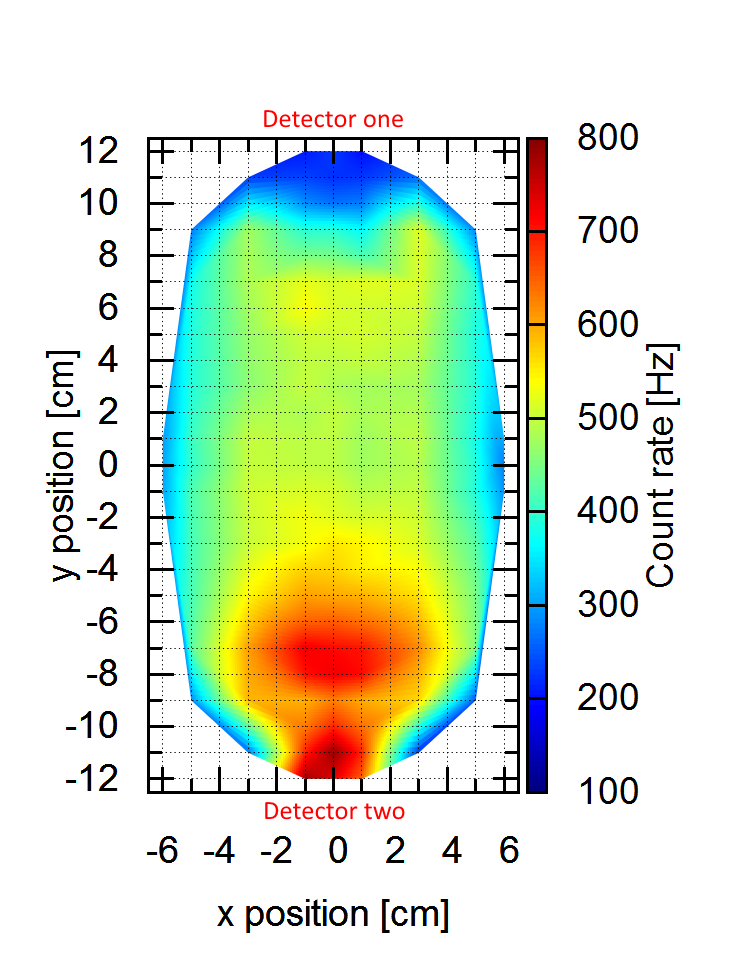
\includegraphics[width=0.24\textwidth]{./plots/spatial/Det2.png}}
	\hfill
	\subfloat[Coincidence rate] {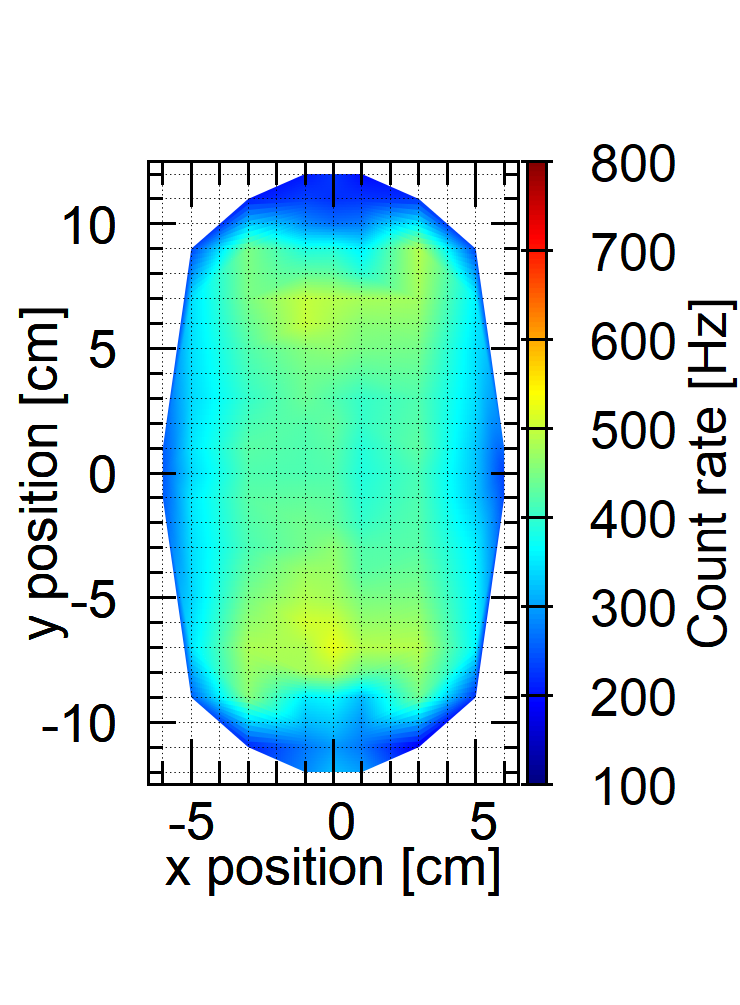
\includegraphics[width=0.24\textwidth]{./plots/spatial/Coinc_large.png}}
	\hfill
	\caption[Efficiency measurement setup]{Efficiency measurement at plastic scintillator with a \sr{} source at different positions. The heat map was plotted with \tit{gnuplot's pm3d} feature, the data between the measurement points was interpolated by the same software. Note that the coincidence count rate in front of one detector is mainly dominated by the count rate of the opposite detector.}
	\label{fig:efficiency}
\end{figure} 




HEATMAP OF COUNTRATE \\
EXPLANATION OF ASYMMETRY \\
TIMING MEASUREMENT \\
ENERGY MEASUREMENT \\
RESUME 





\bibliographystyle{plain}
\bibliography{./bib}


\end{document}  